\documentclass{beamer}

\mode<presentation> {
  
  % The Beamer class comes with a number of default slide themes
  % which change the colors and layouts of slides. Below this is a list
  % of all the themes, uncomment each in turn to see what they look like.
  
  \usetheme{default}
  %\usetheme{AnnArbor}
  %\usetheme{Antibes}
  %\usetheme{Bergen}
  %\usetheme{Berkeley}
  %\usetheme{Berlin}
  %\usetheme{Boadilla}
  %\usetheme{CambridgeUS}
  %\usetheme{Copenhagen}
  %\usetheme{Darmstadt}
  %\usetheme{Dresden}
  %\usetheme{Frankfurt}
  %\usetheme{Goettingen}
  %%\usetheme{Hannover}
  %\usetheme{Ilmenau}
  %\usetheme{JuanLesPins}
  %\usetheme{Luebeck}
  %\usetheme{Madrid}
  %\usetheme{Malmoe}
  %\usetheme{Marburg}
  %\usetheme{Montpellier}
  %\usetheme{PaloAlto}
  %\usetheme{Pittsburgh}
  %\usetheme{Rochester}
  %\usetheme{Singapore}
  %\usetheme{Szeged}
  %\usetheme{Warsaw}
  
  
  
  % As well as themes, the Beamer class has a number of color themes
  % for any slide theme. Uncomment each of these in turn to see how it
  % changes the colors of your current slide theme.
  
  %\usecolortheme{albatross}
  %\usecolortheme{beaver}
  \usecolortheme{beetle}
  %\usecolortheme{crane}
  %\usecolortheme{dolphin}
 % \usecolortheme{dove}
  %\usecolortheme{fly}
  %\usecollortheme{froggy}
  %\usecolortheme{lily}
  %\usecolortheme{orchid}
  %\usecolortheme{rose}
  %\usecolortheme{seagull}
  %\usecolortheme{seahorse}
  %\usecolortheme{whale}
  %\usecolortheme{wolverine}
  
  %\setbeamertemplate{footline} % To remove the footer line in all slides uncomment this line
  %\setbeamertemplate{footline}[page number] % To replace the footer line in all slides with a simple slide count uncomment this line
  
  %\setbeamertemplate{navigation symbols}{} % To remove the navigation symbols from the bottom of all slides uncomment this line
}

\usepackage{graphicx} % Allows including images
\usepackage{booktabs}
\usepackage{media9}
\usepackage{hyperref}
%\usepackage{rmannot}
%\usepackage{yt4pdf}
% Allows the use of \toprule, \midrule and \bottomrule in tables

%----------------------------------------------------------------------------------------
  %  TITLE PAGE
%----------------------------------------------------------------------------------------
  
  \title[Cisek (1999)]{Beyond the computer metaphor:\\ Behavior as interaction.\\Cisek (1999)} % The short title appears at the bottom of every slide, the full title is only on the title page

\author{Nathan A. Baune} % Your name
\institute[UM] % Your institution as it will appear on the bottom of every slide, may be shorthand to save space
{
  University of Missouri-Columbia   \\   % Your institution for the title page
  \medskip
   \textit{} %  class
}
\titlegraphic{\includegraphics[width=1.5cm]{mizzouemblem.png}%\hspace*{4.75cm}~%
   % \includegraphics[width=2cm]{mizzouemblem.png}
    }
\date{\today} % Date, can be changed to a custom date

\begin{document}

%1

%\begin{frame}
%\frametitle{Overview} % Table of contents slide, comment this block out to remove it
%\tableofcontents % Throughout your presentation, if you choose to use \section{} and \subsection{} commands, these will automatically be printed on this slide as an overview of your presentation
%\end{frame}


%----------------------------------------------------------------------------------------
  %  PRESENTATION SLIDES
%----------------------------------------------------------------------------------------
\section{}

\begin{frame}
\frametitle{Overview}
\begin{tabular}{lc}
Group& N\\
\hline
Control&14\\
Amputee&22\\
Transplant&4\footnote{6 counting DR's 3 sessions}\\
Replant&4\\
\hline
\end{tabular}
\end{frame}


\begin{frame}
\frametitle{Controls and Replant/Transplant Patients by Participant}
\begin{figure}
\setlength{\fboxsep}{0pt}%
\setlength{\fboxrule}{1pt}%
\fbox{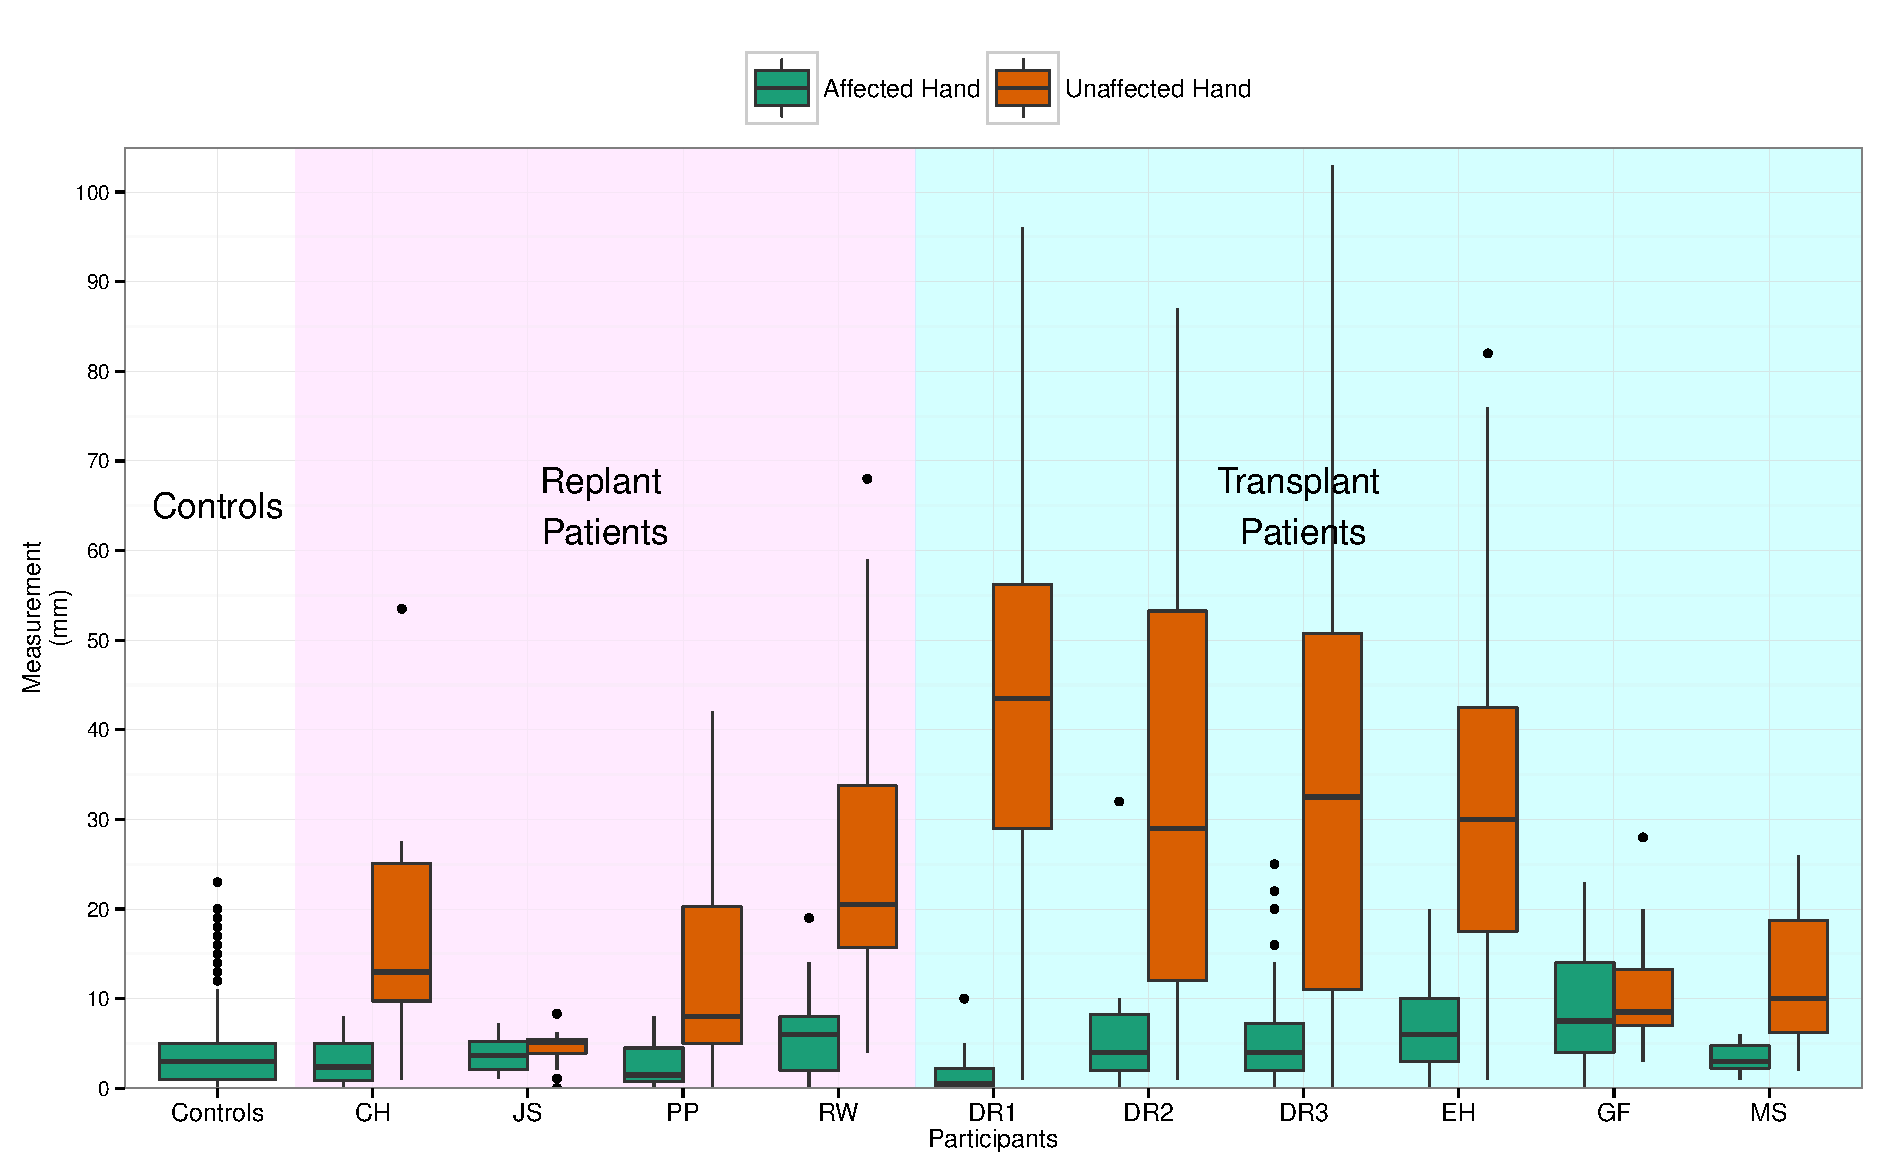
\includegraphics[width= 10cm]{boxplot_patientcontrols.pdf}}
\end{figure}
\tiny
The upper and lower "hinges" correspond to the first and third quartiles (the 25th and 75th percentiles). The upper whisker extends from the hinge to the highest value that is within 1.5 * IQR of the hinge, where IQR is the inter-quartile range, or distance between the first and third quartiles. The lower whisker extends from the hinge to the lowest value within 1.5 * IQR of the hinge. Data beyond the end of the whiskers are outliers and plotted as points (as specified by Tukey).
\end{frame}

\begin{frame}
\frametitle{Amputees by Participant}
\begin{figure}
\setlength{\fboxsep}{0pt}%
\setlength{\fboxrule}{1pt}%
\fbox{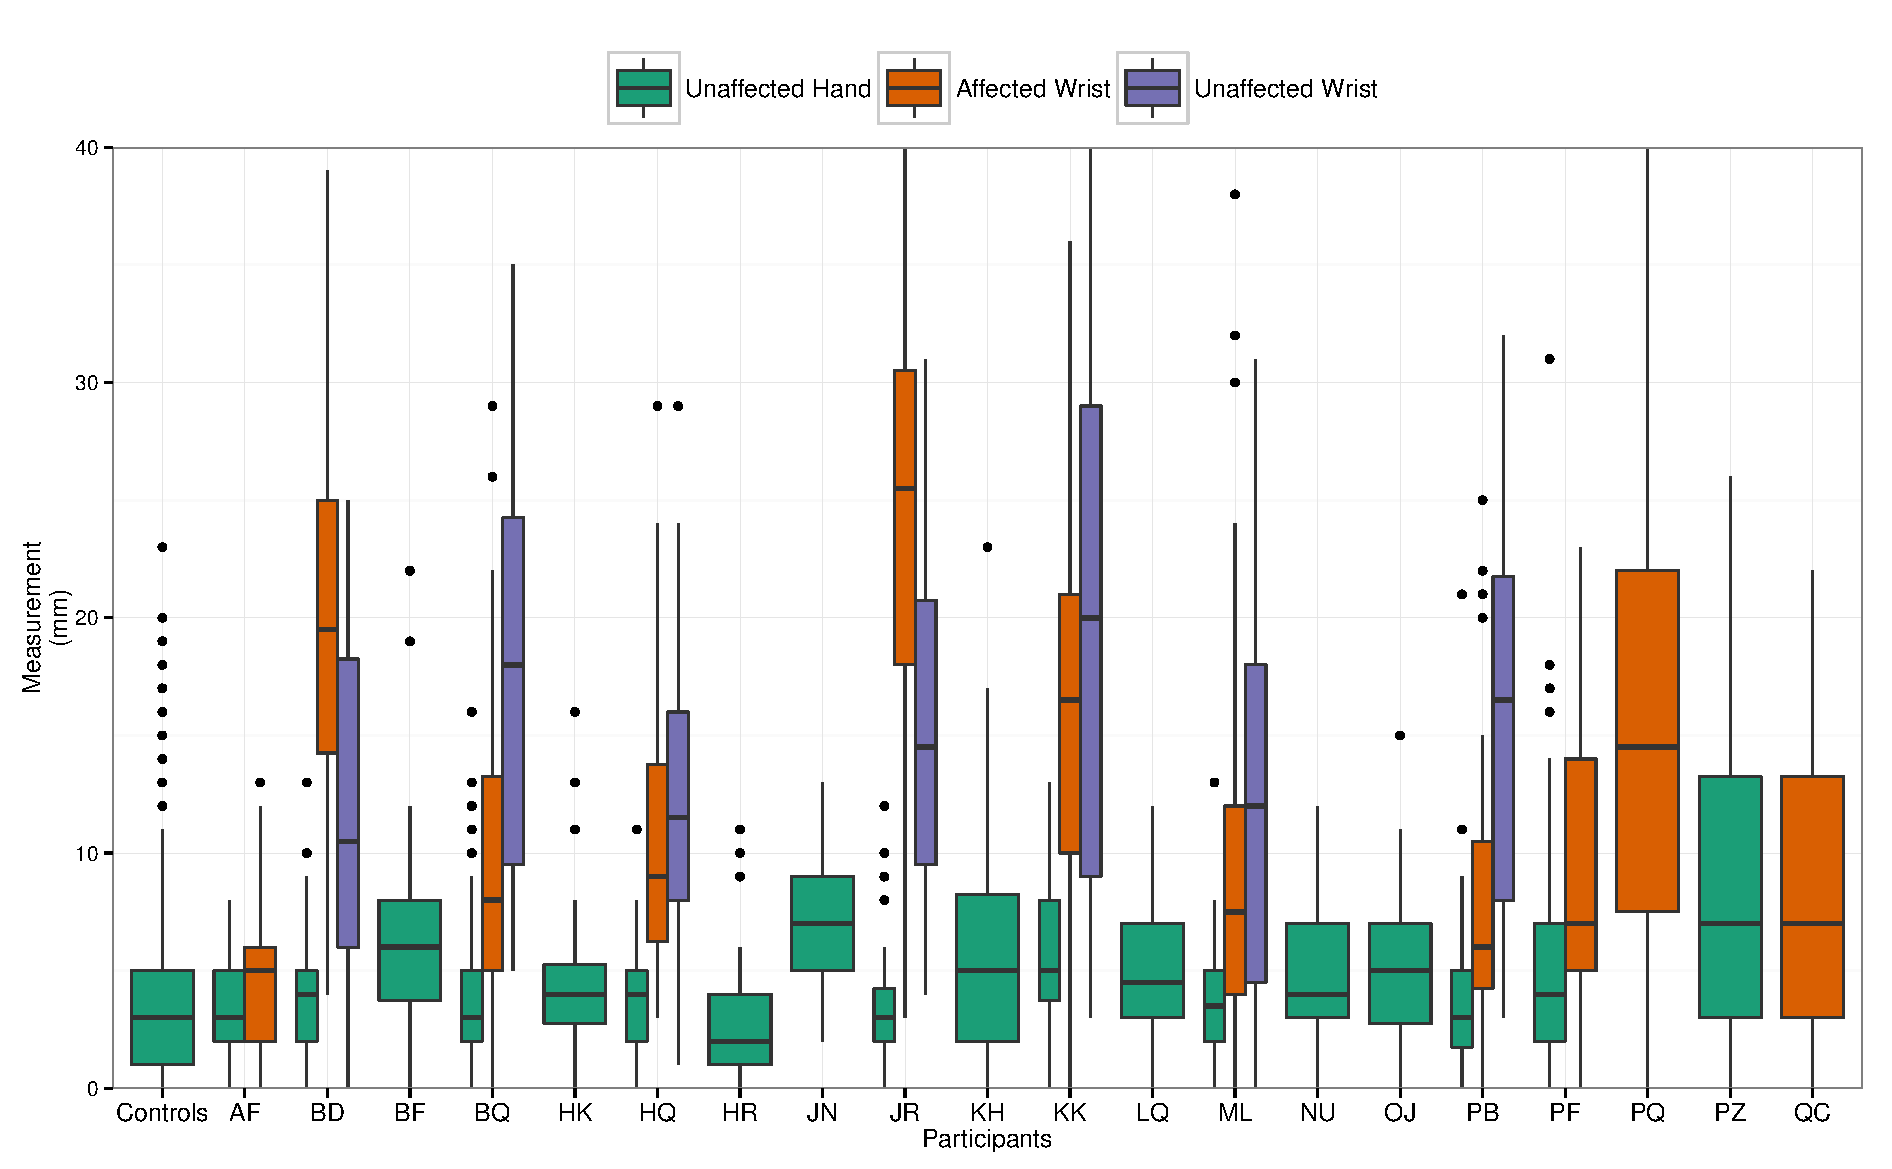
\includegraphics[width= 10cm]{boxplot_amputees.pdf}}
\end{figure}
\tiny
The upper and lower "hinges" correspond to the first and third quartiles (the 25th and 75th percentiles). The upper whisker extends from the hinge to the highest value that is within 1.5 * IQR of the hinge, where IQR is the inter-quartile range, or distance between the first and third quartiles. The lower whisker extends from the hinge to the lowest value within 1.5 * IQR of the hinge. Data beyond the end of the whiskers are outliers and plotted as points (as specified by Tukey).
\end{frame}

\begin{frame}
\frametitle{Comparison Amputees vs. Replant/Transplant Patients\footnote{same control group in both graphs}}
\begin{figure}
\setlength{\fboxsep}{0pt}%
\setlength{\fboxrule}{1pt}%
\fbox{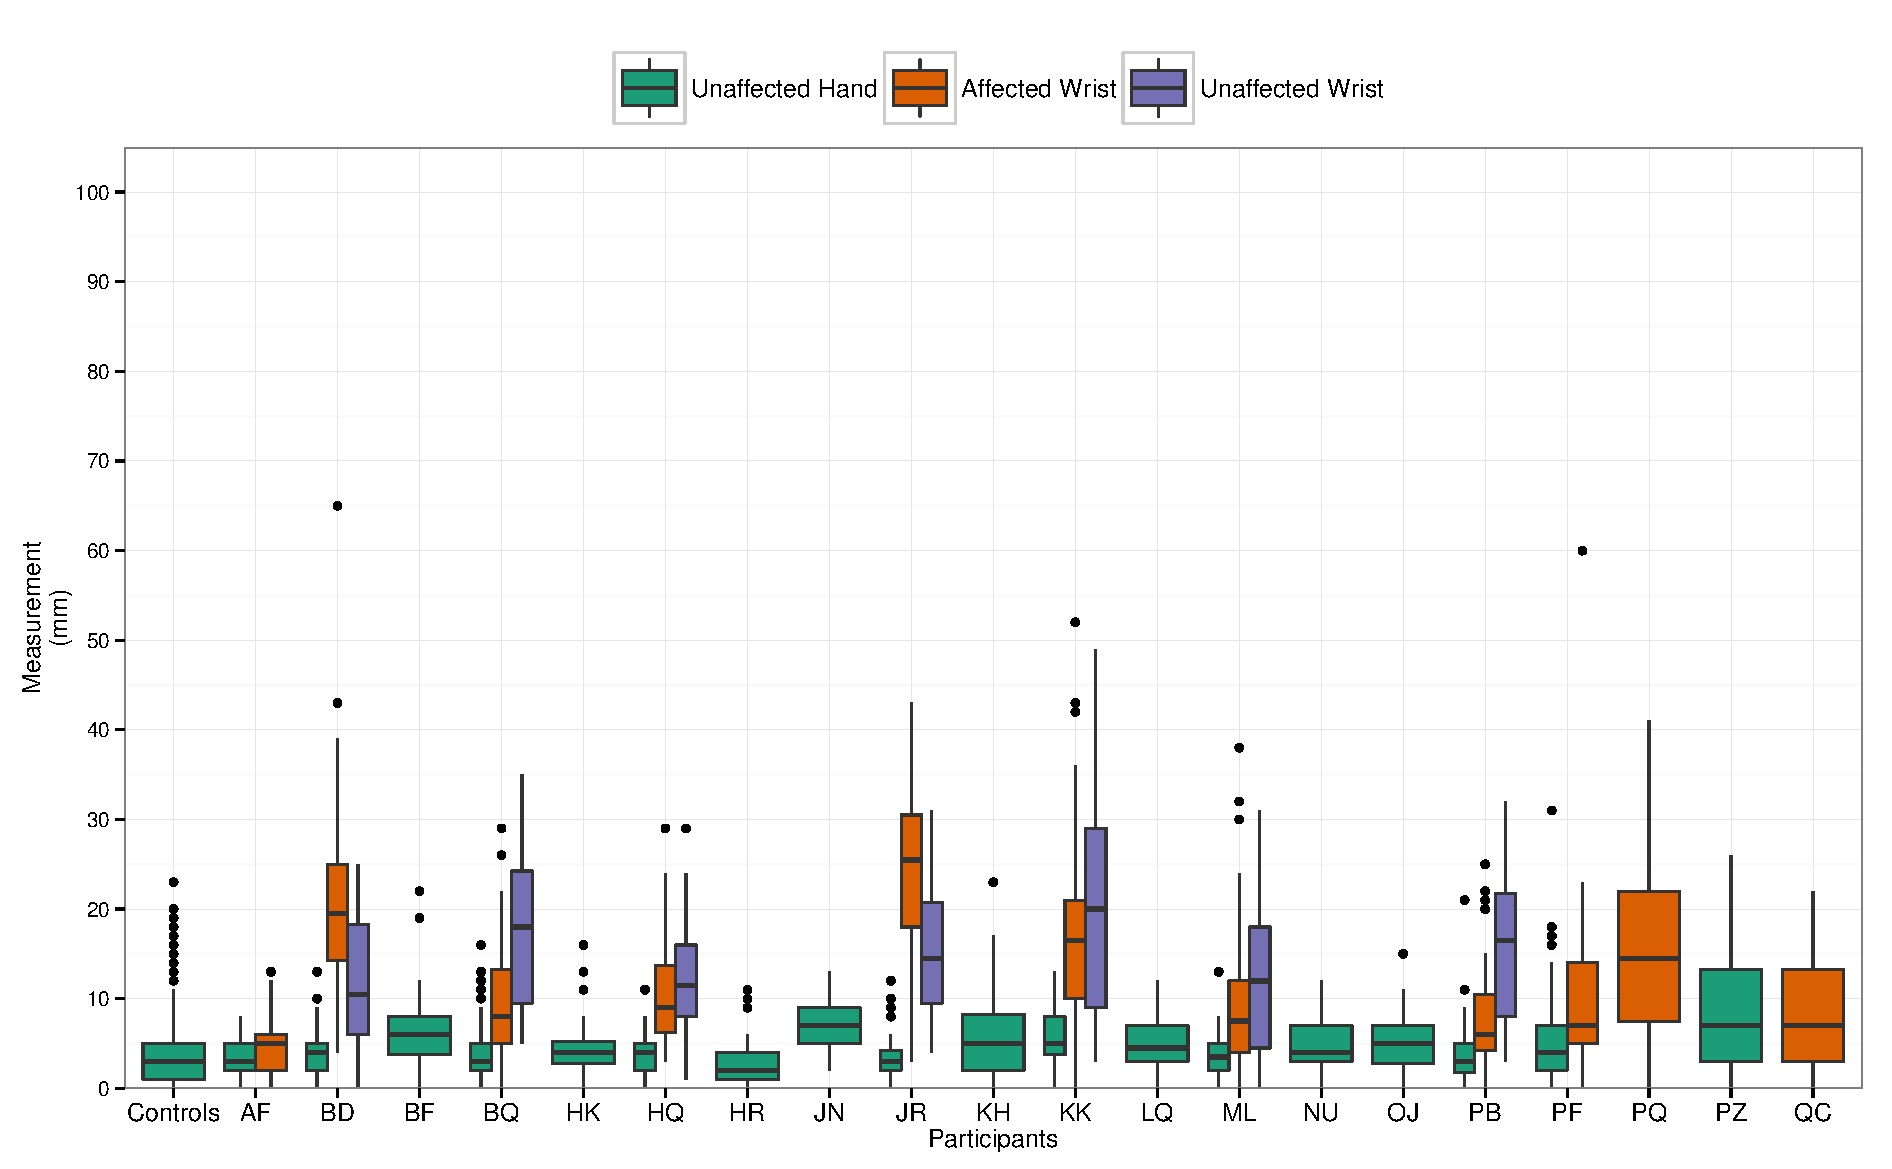
\includegraphics[width= 6.3cm]{boxplot_amputees_comparison.pdf}}
\end{figure}
\vspace{-25pt}
\begin{figure}
\setlength{\fboxsep}{0pt}%
\setlength{\fboxrule}{1pt}%
\fbox{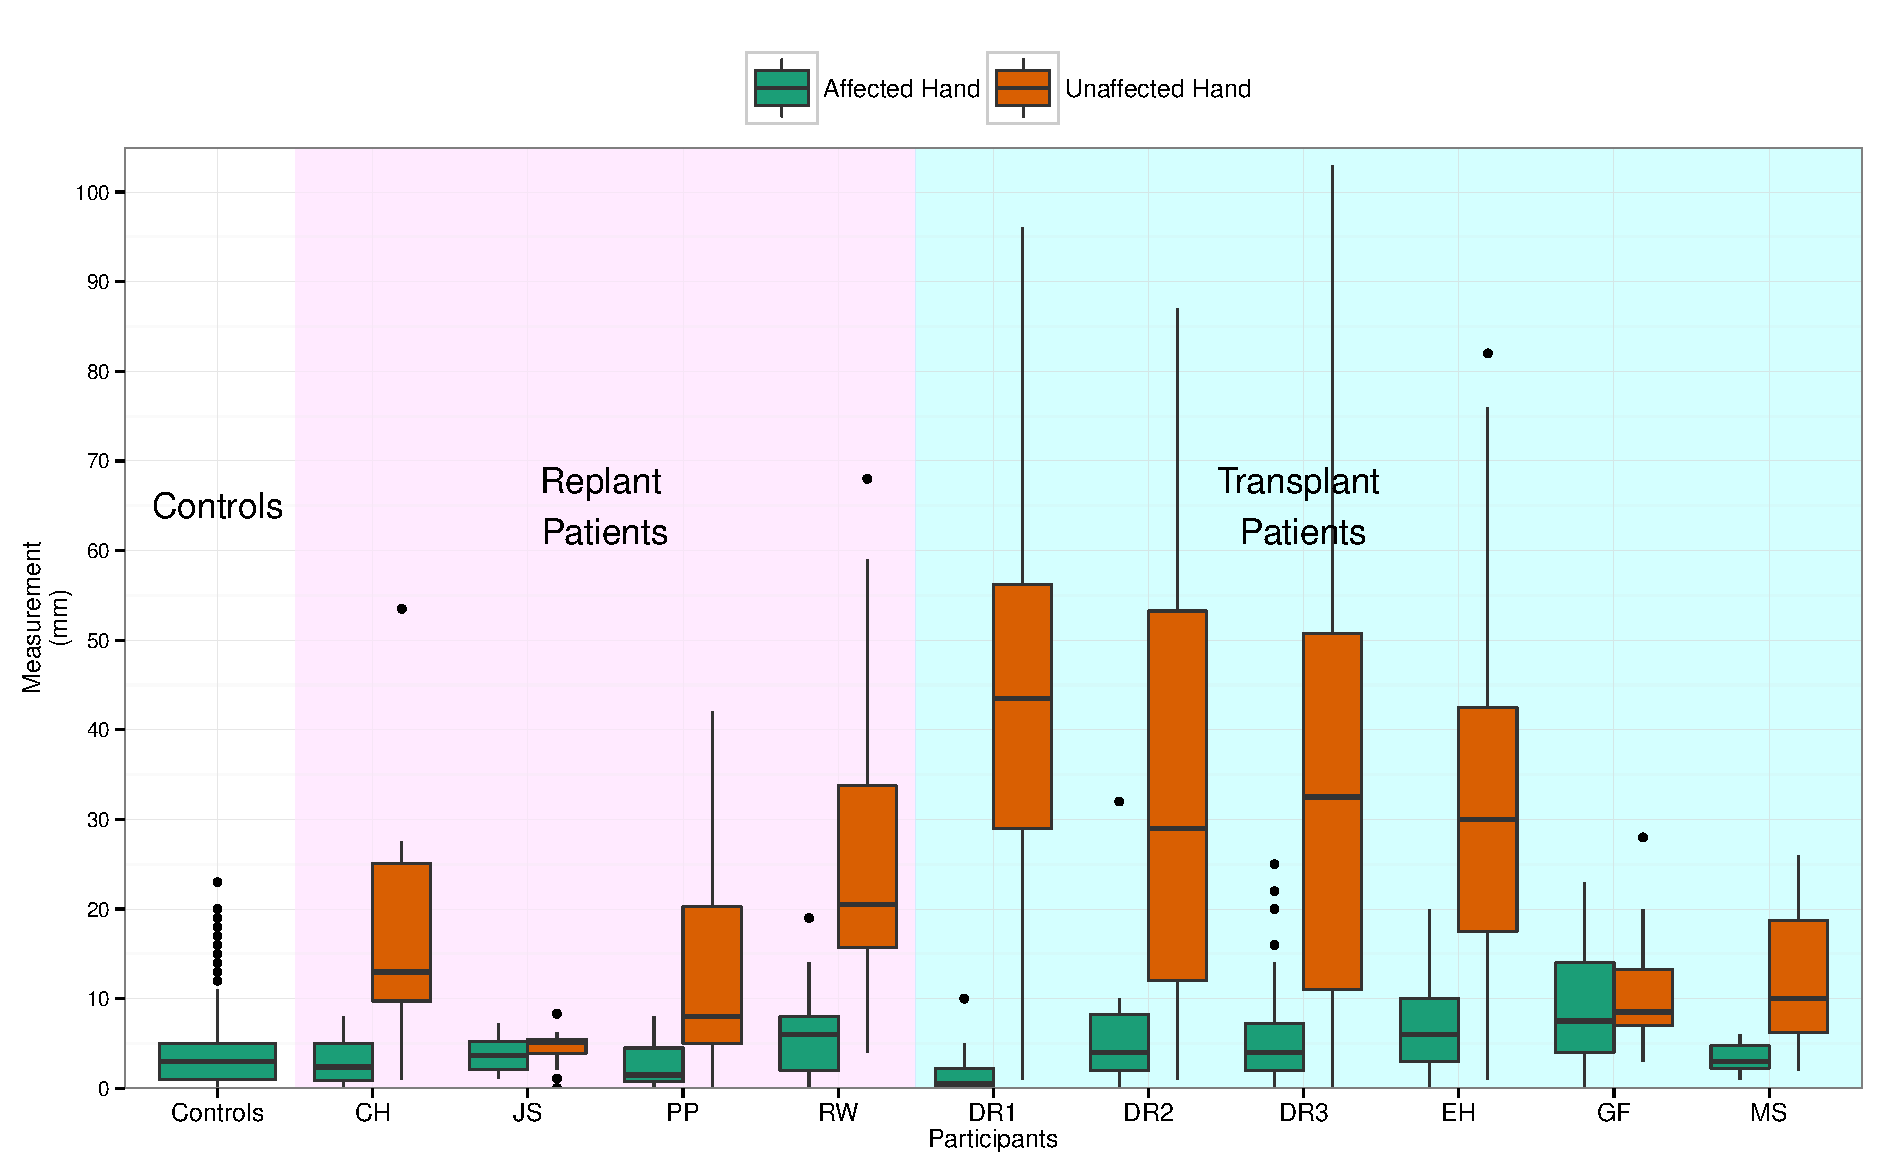
\includegraphics[width= 6.3cm]{boxplot_patientcontrols.pdf}}
\end{figure}
\end{frame}

\begin{frame}
\frametitle{Controls, Amputees, and Replant/Transplant Patients by Group}
\begin{figure}
\setlength{\fboxsep}{0pt}%
\setlength{\fboxrule}{1pt}%
\fbox{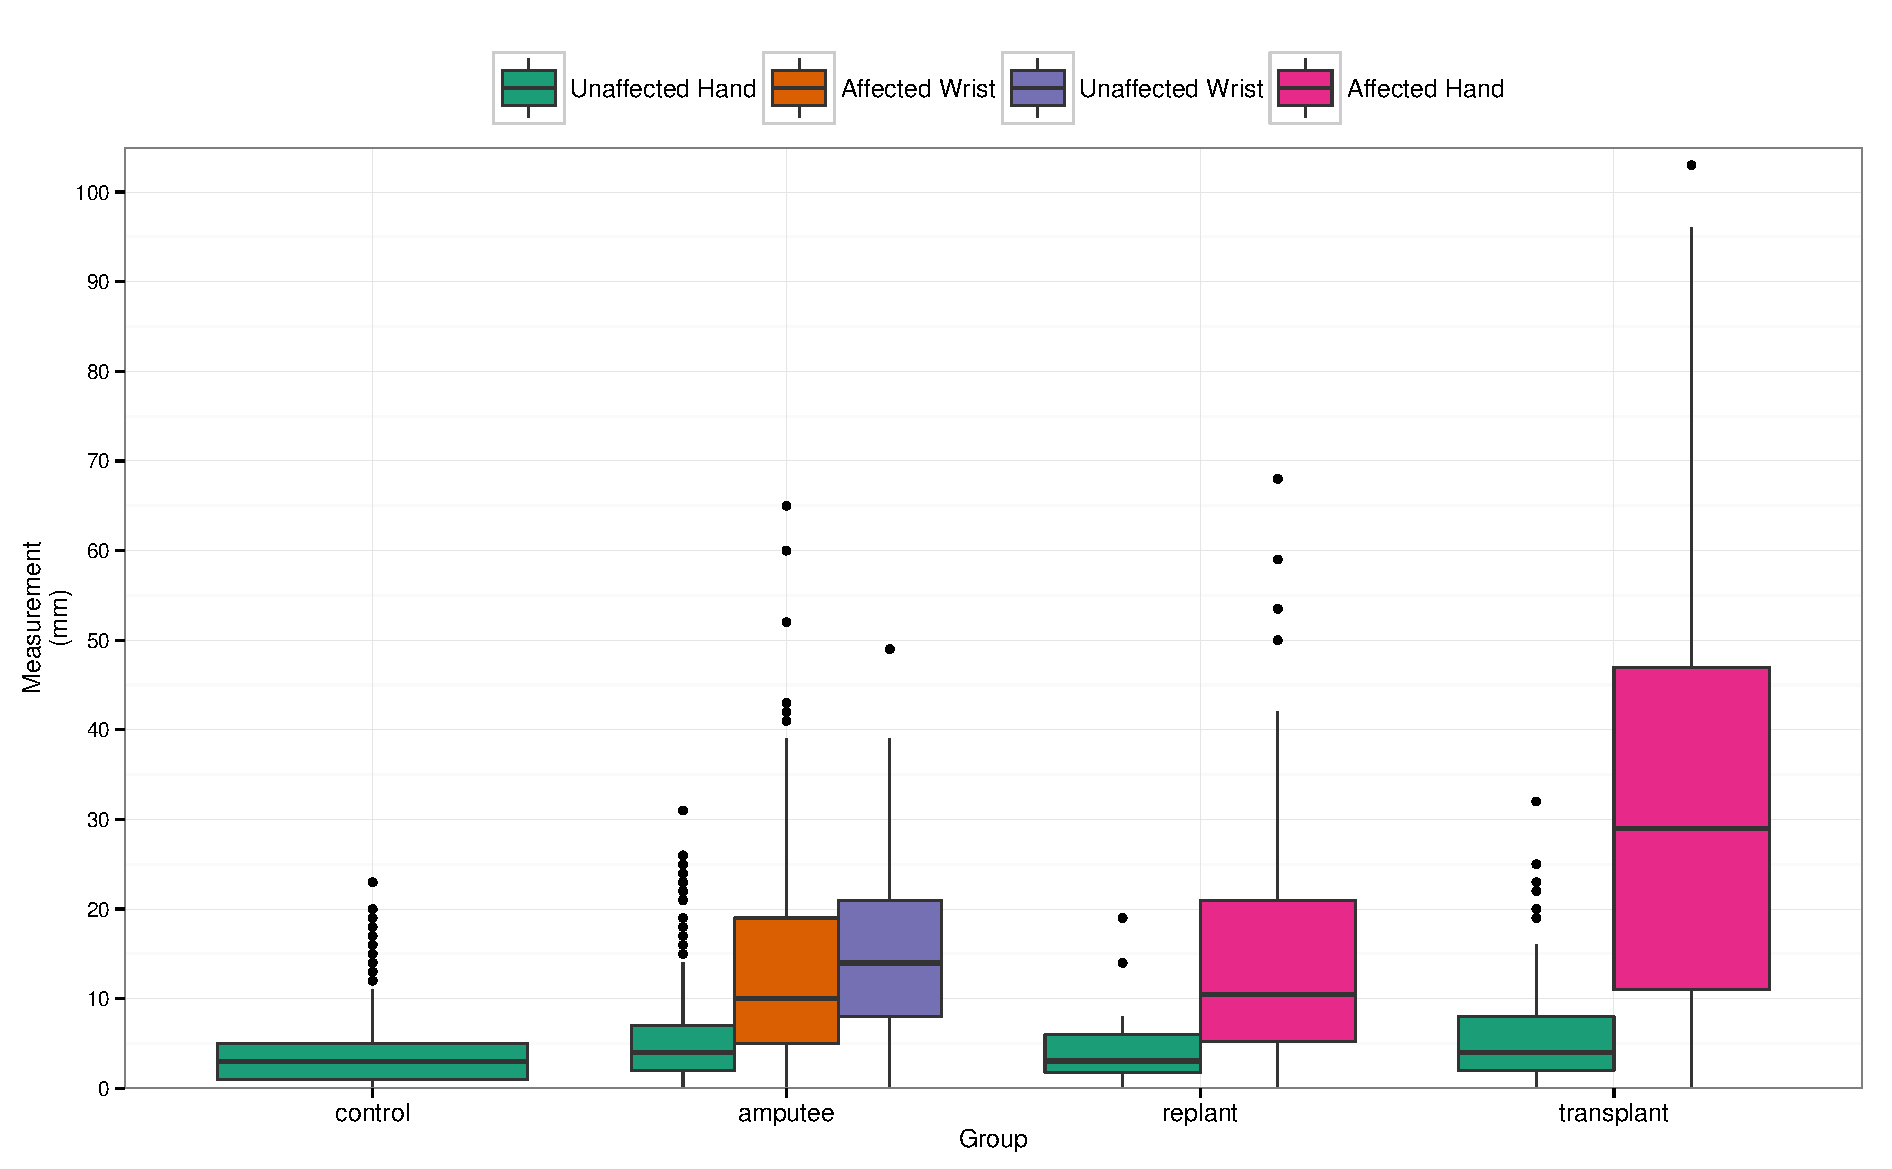
\includegraphics[width= 10cm]{boxplot_mmbygroup.pdf}}
\end{figure}
\tiny
The upper and lower "hinges" correspond to the first and third quartiles (the 25th and 75th percentiles). The upper whisker extends from the hinge to the highest value that is within 1.5 * IQR of the hinge, where IQR is the inter-quartile range, or distance between the first and third quartiles. The lower whisker extends from the hinge to the lowest value within 1.5 * IQR of the hinge. Data beyond the end of the whiskers are outliers and plotted as points (as specified by Tukey).
\end{frame}

\begin{frame}
\frametitle{Replant/Transplant Patients by Location}
\begin{columns}[T]
\begin{column}{.7\textwidth}
\begin{figure}
\setlength{\fboxsep}{0pt}%
\setlength{\fboxrule}{1pt}%
\fbox{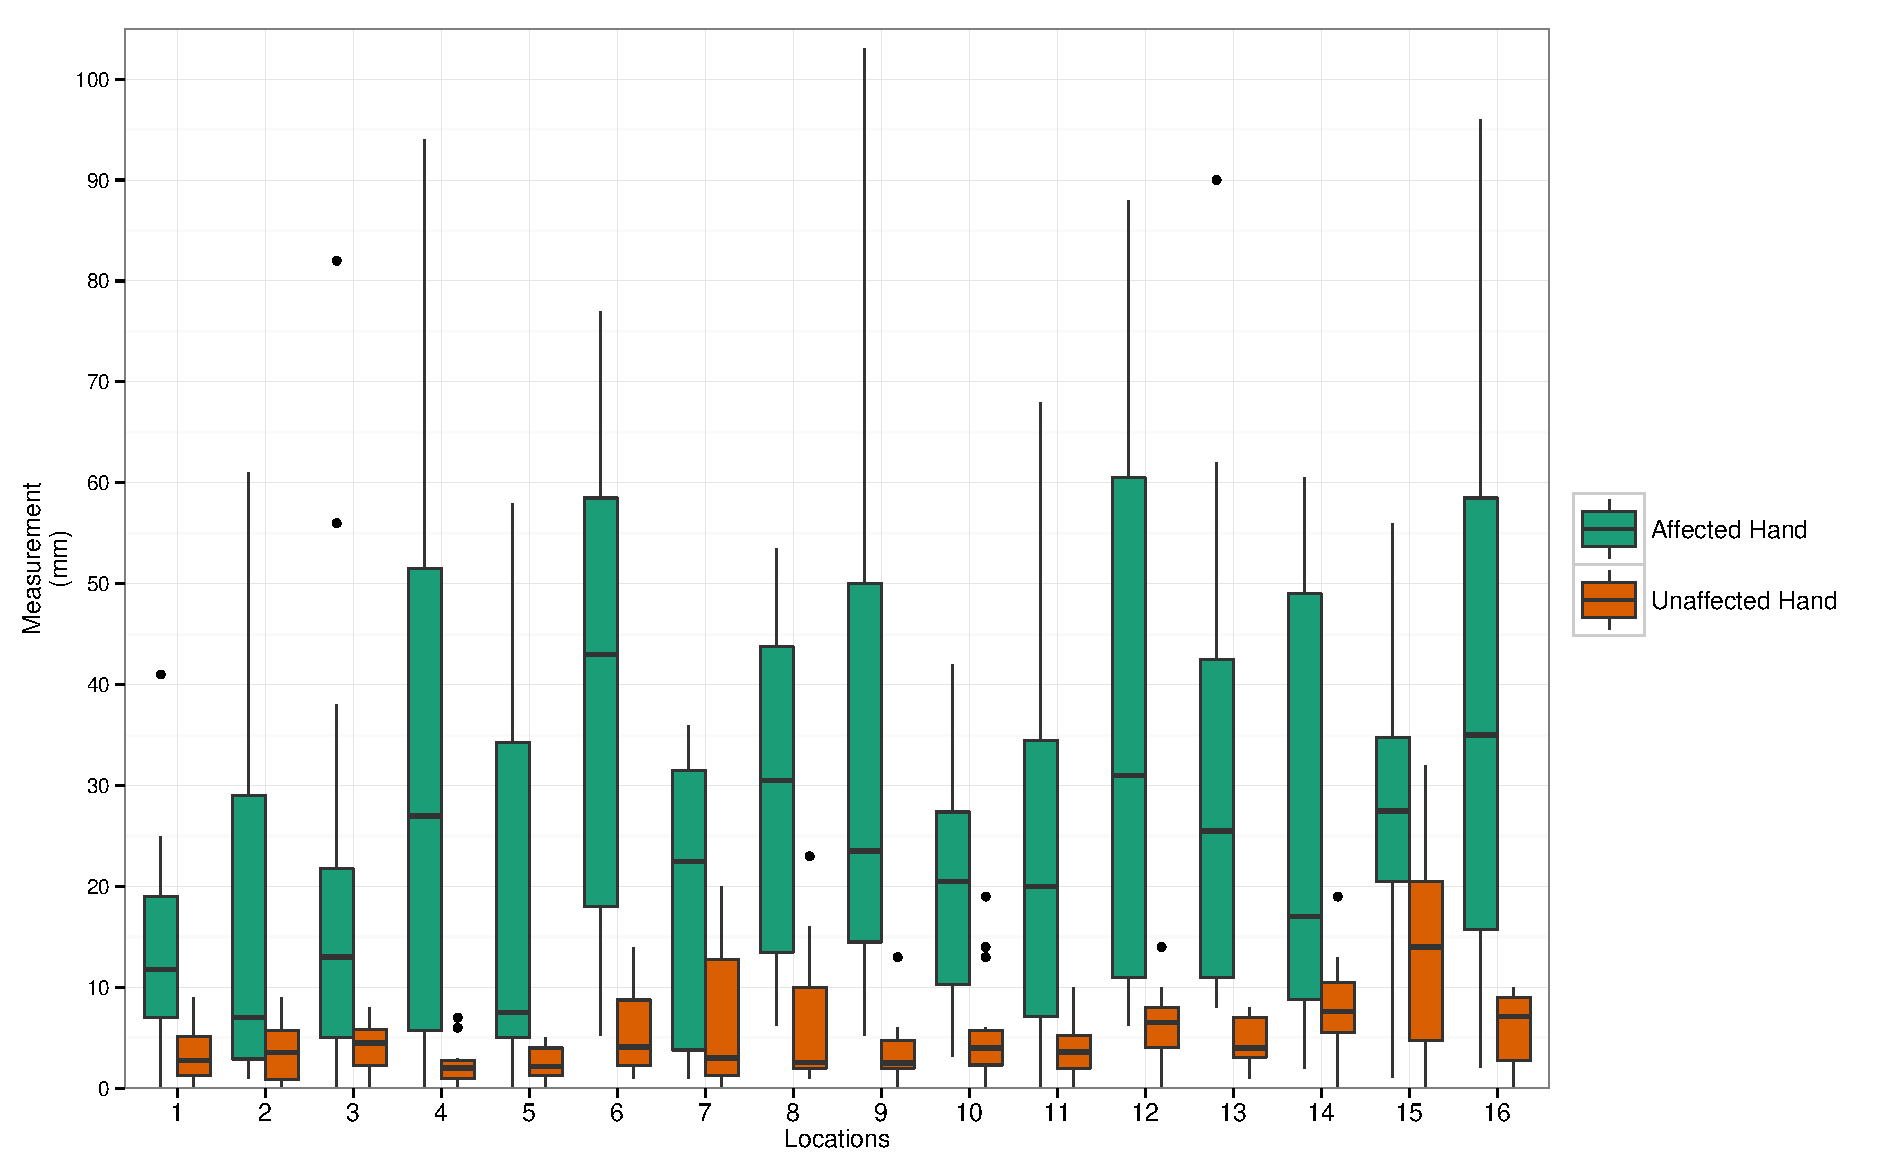
\includegraphics[width= 8.cm]{patient_location_mm.pdf}}
\end{figure}
\end{column}

\begin{column}{.3\textwidth}
\begin{figure}
\setlength{\fboxsep}{0pt}%
\setlength{\fboxrule}{1pt}%
\fbox{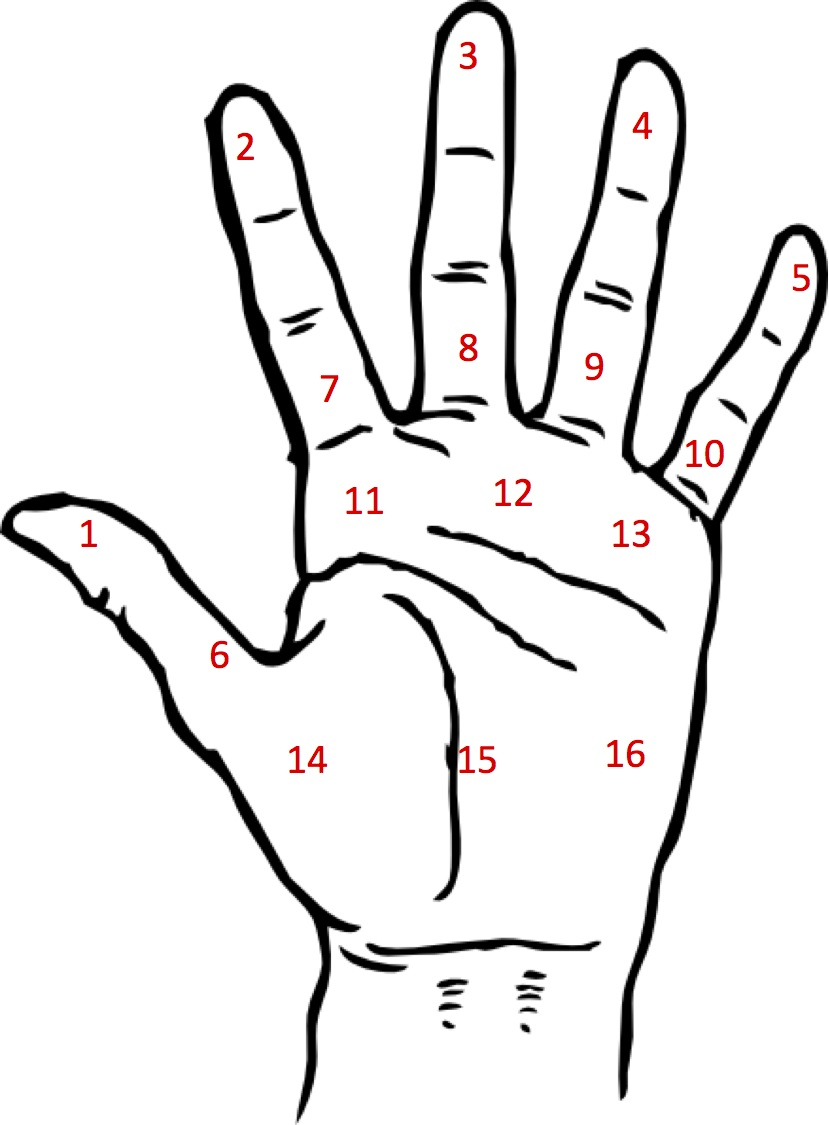
\includegraphics[width= 3.cm]{HandLocs_Left.jpg}}
\end{figure}
\end{column}
\end{columns}
\end{frame}

\begin{frame}
\frametitle{Controls by Location}
\begin{columns}[T]
\begin{column}{.7\textwidth}
\begin{figure}
\setlength{\fboxsep}{0pt}%
\setlength{\fboxrule}{1pt}%
\fbox{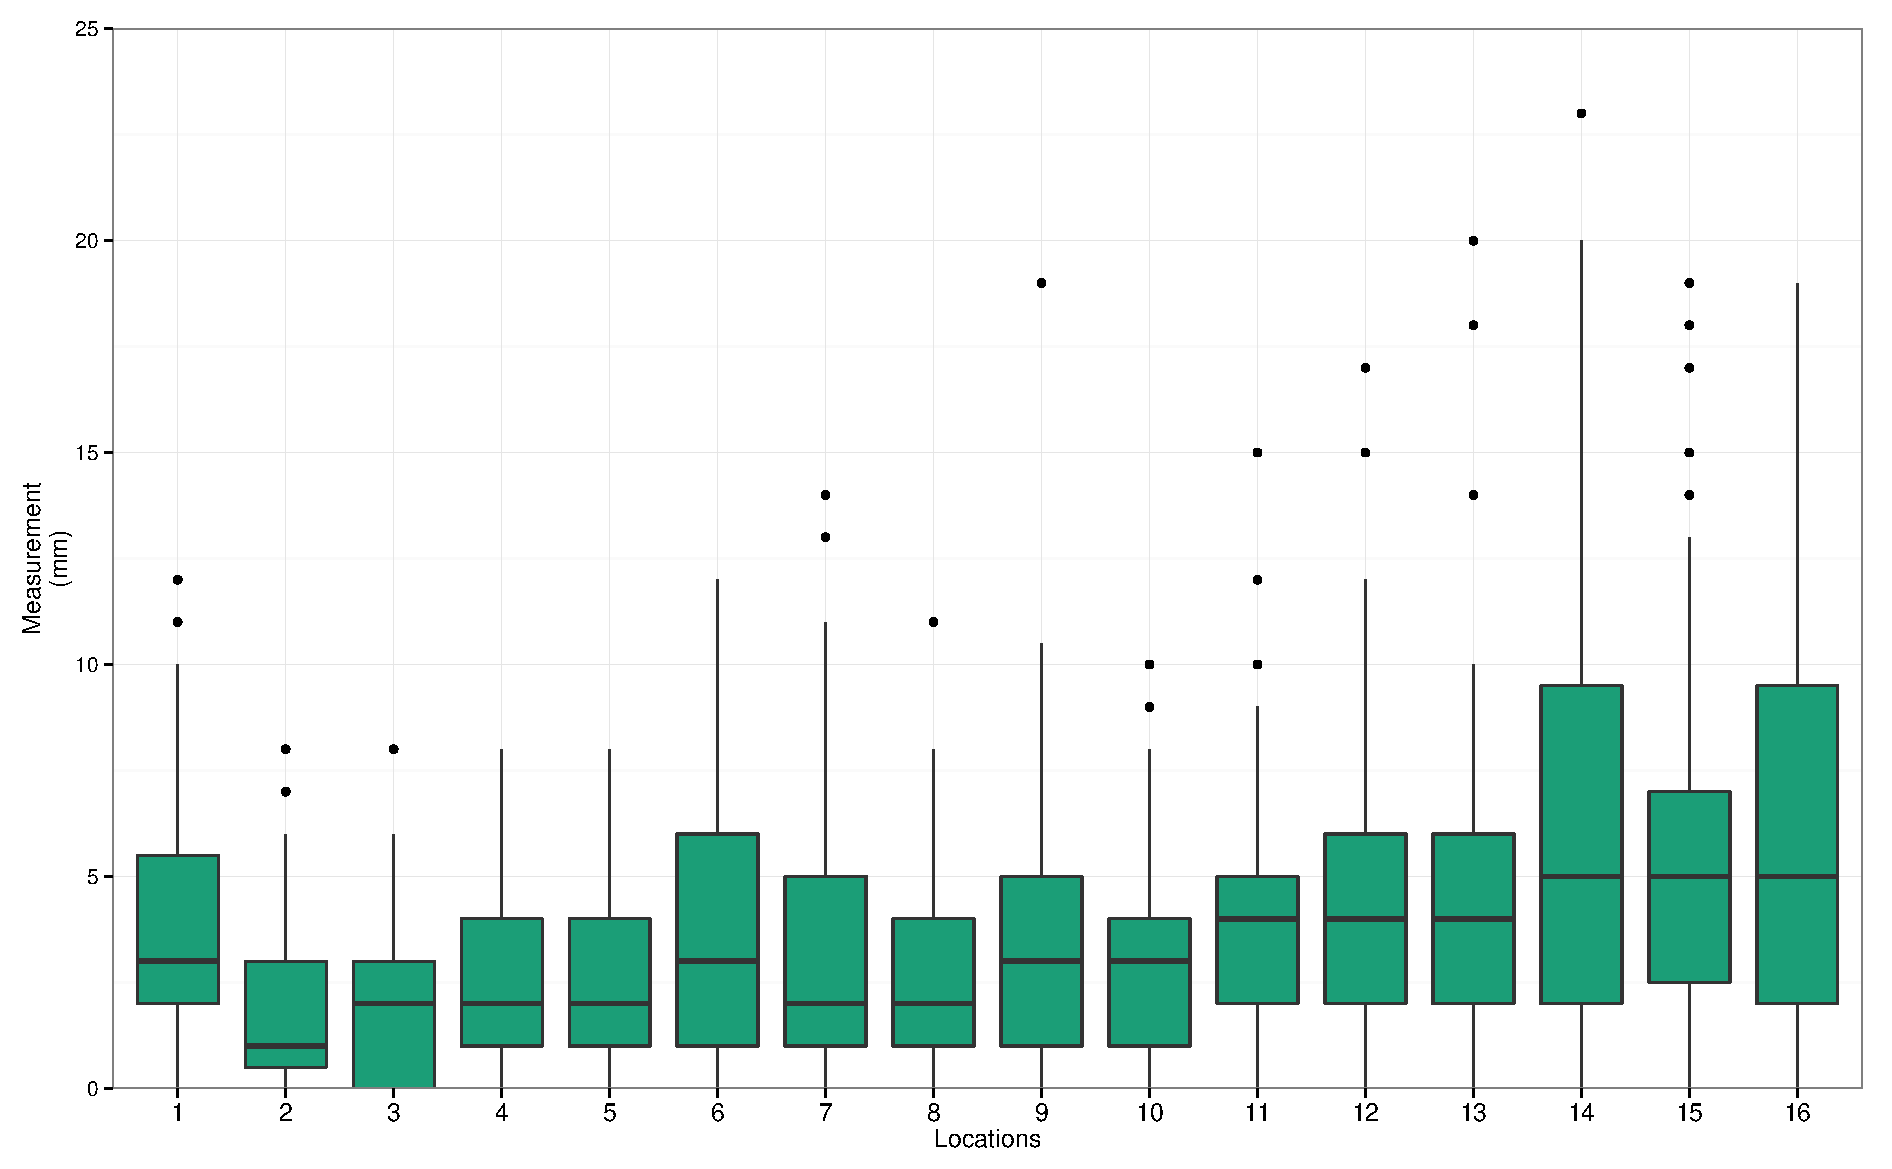
\includegraphics[width= 8.cm]{control_location_mm.pdf}}
\end{figure}
\end{column}

\begin{column}{.3\textwidth}
\begin{figure}
\setlength{\fboxsep}{0pt}%
\setlength{\fboxrule}{1pt}%
\fbox{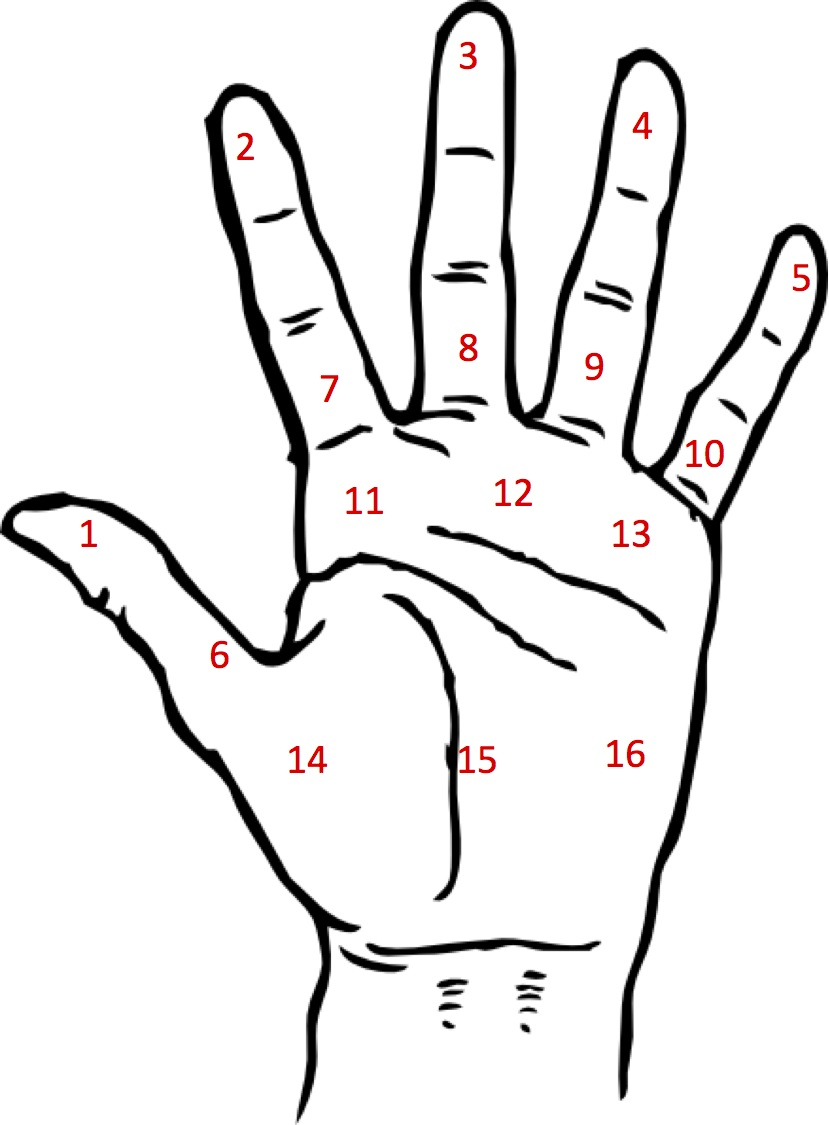
\includegraphics[width= 3.cm]{HandLocs_Left.jpg}}
\end{figure}
\end{column}
\end{columns}
\end{frame}

%comparison of the two
\begin{frame}
\frametitle{Location Comparison}
\begin{columns}[T]
\begin{column}{.7\textwidth}
\begin{figure}
\setlength{\fboxsep}{0pt}%
\setlength{\fboxrule}{1pt}%
\fbox{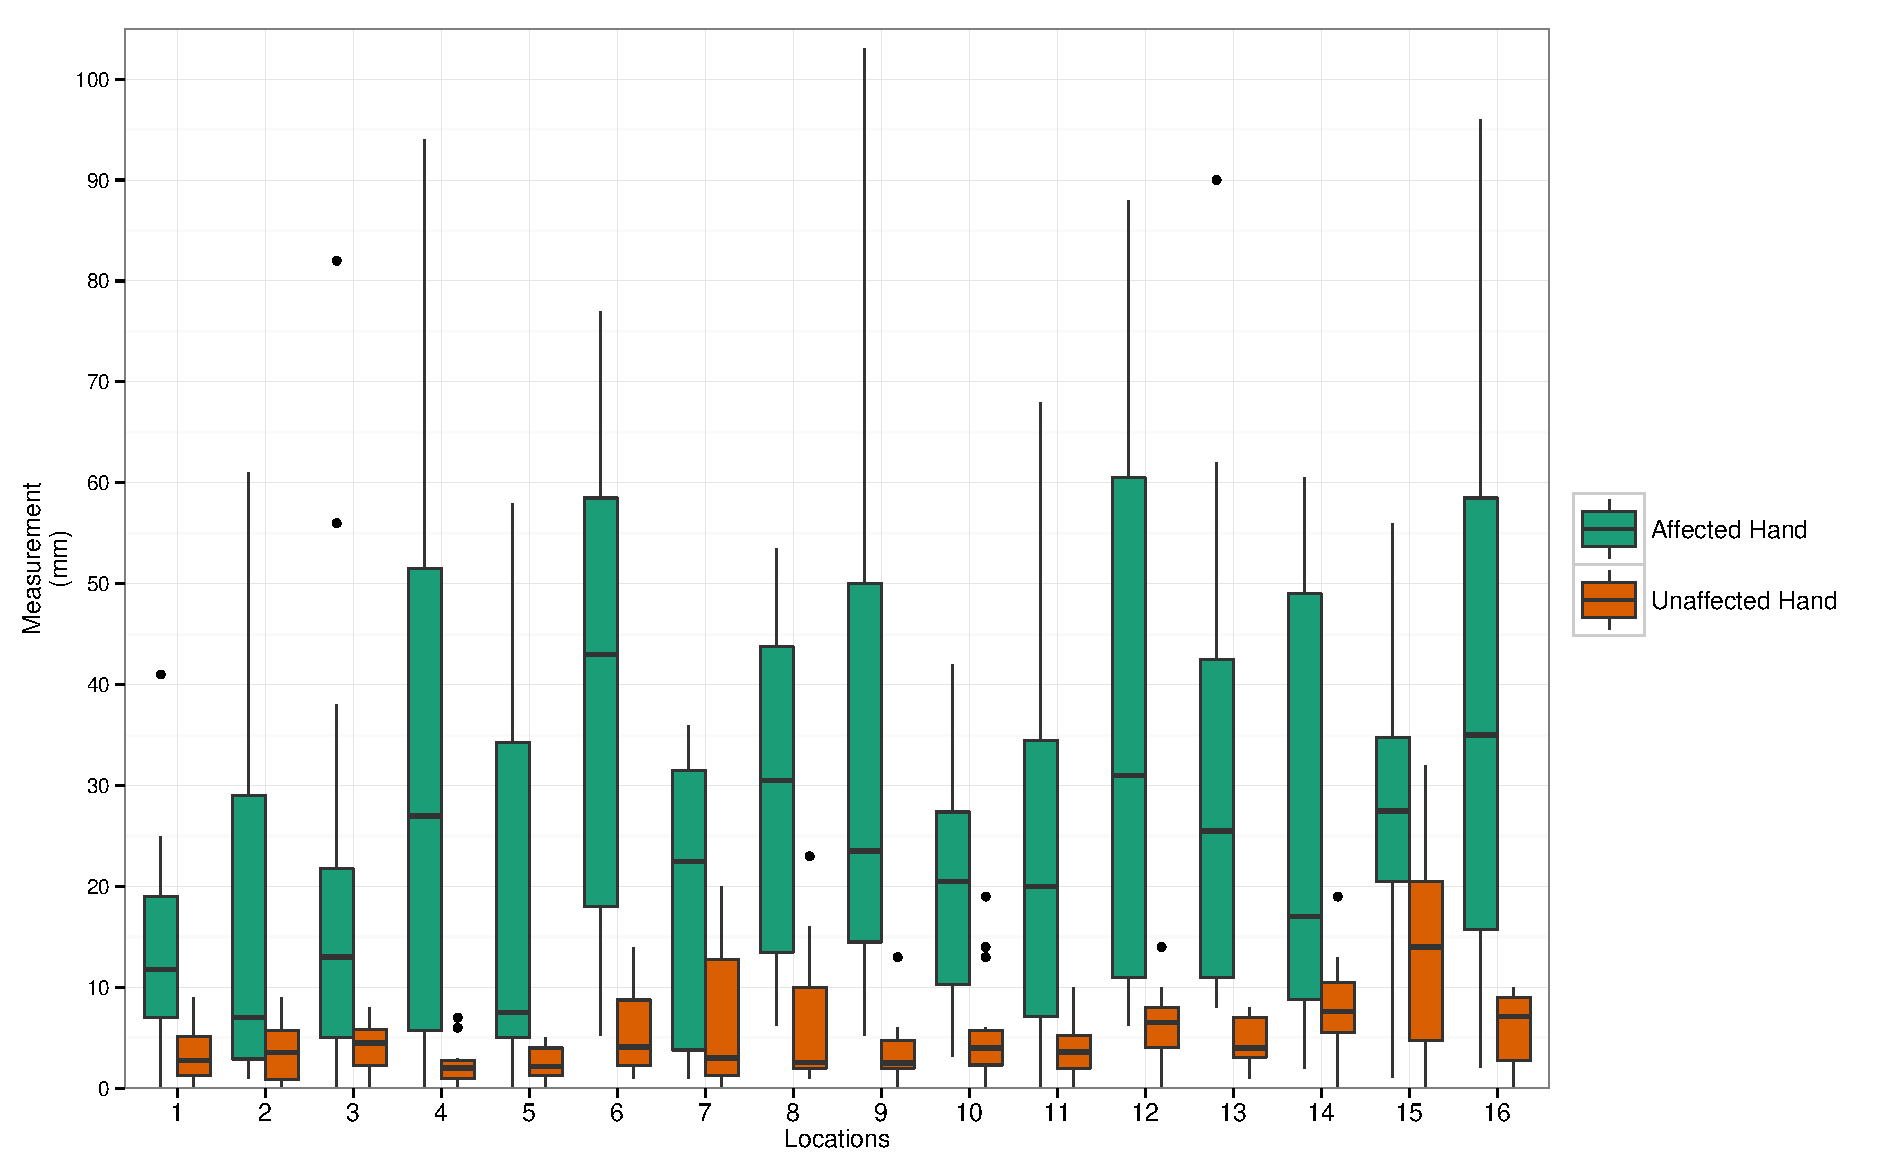
\includegraphics[width= 6.3cm]{patient_location_mm.pdf}}
\end{figure}
\vspace{-25pt}
\begin{figure}
\setlength{\fboxsep}{0pt}%
\setlength{\fboxrule}{1pt}%
\fbox{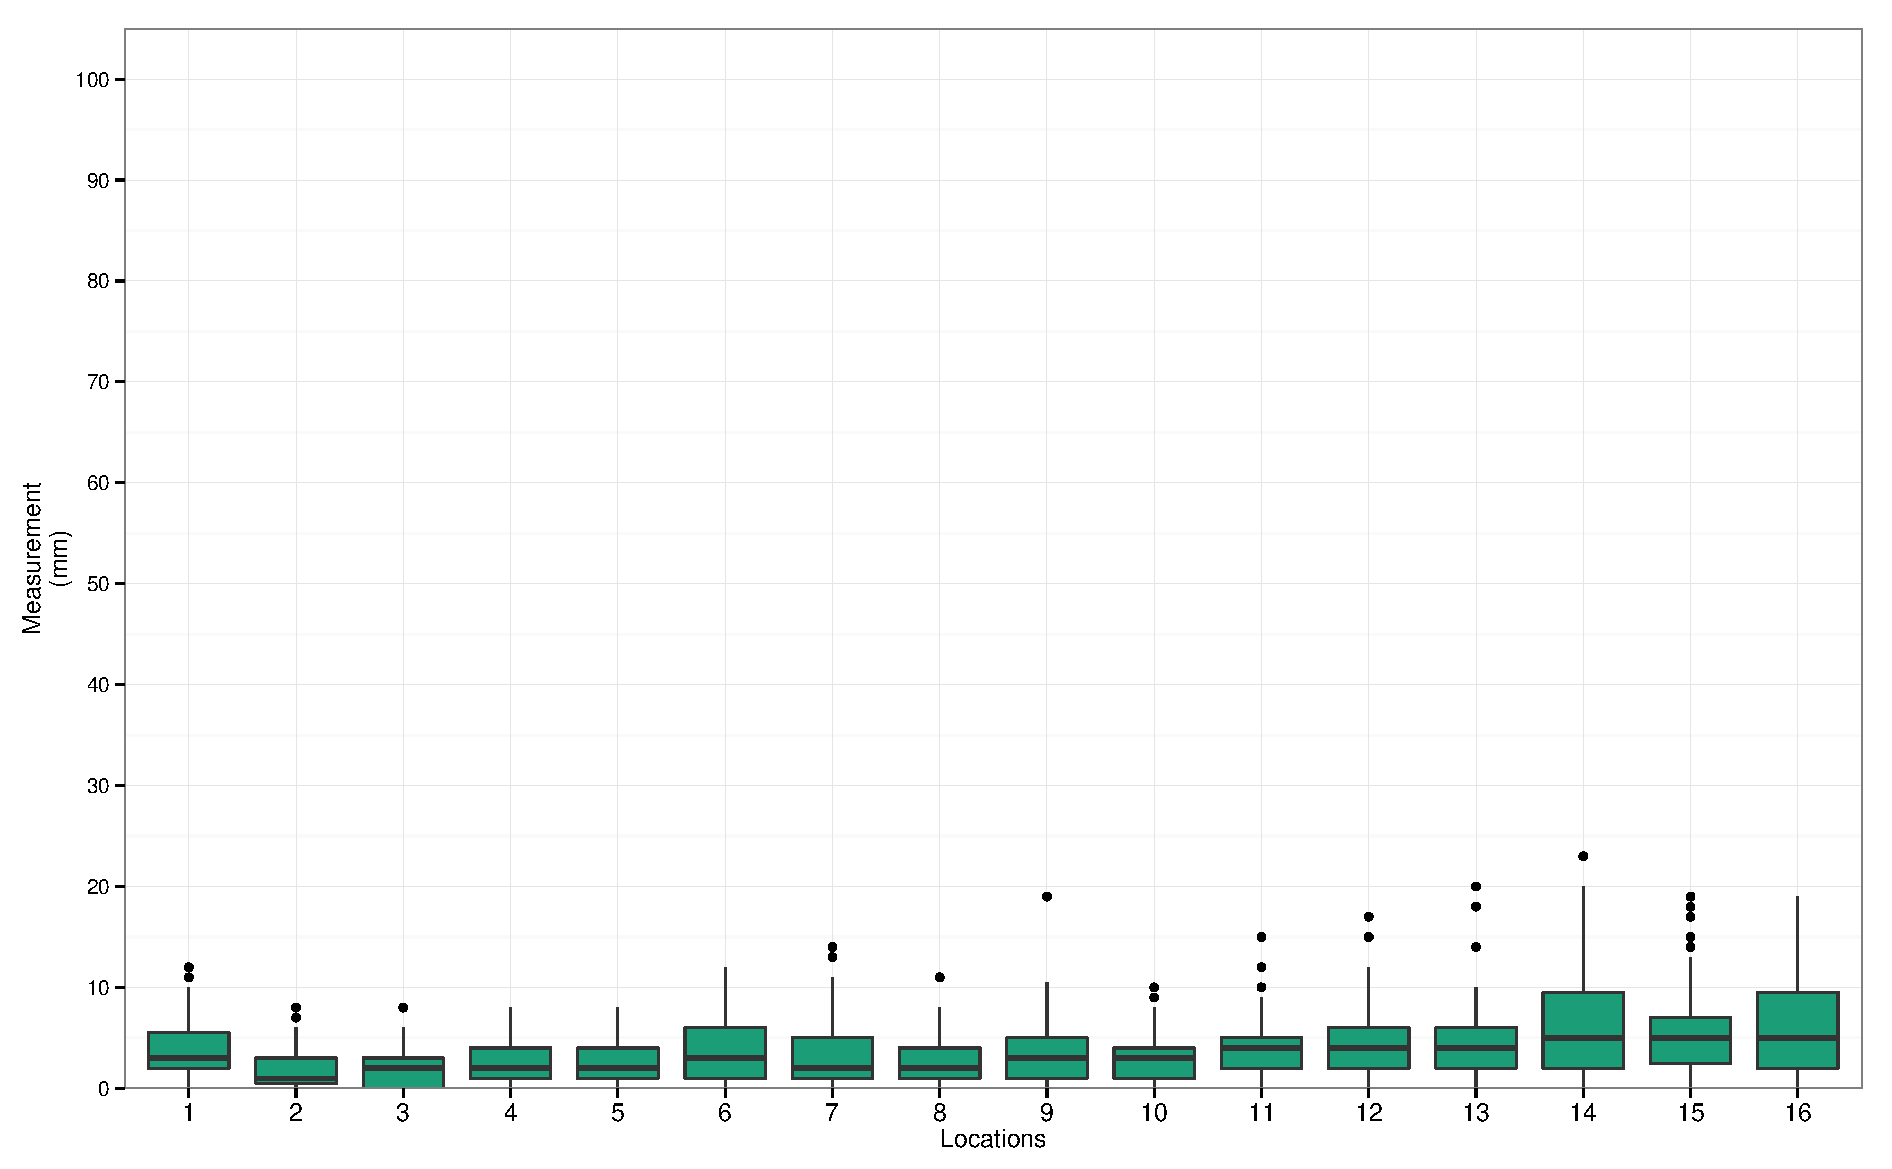
\includegraphics[width= 6.3cm]{control_location_largescale.pdf}}
\end{figure}
\end{column}

\begin{column}{.3\textwidth}
\begin{figure}
\setlength{\fboxsep}{0pt}%
\setlength{\fboxrule}{1pt}%
\fbox{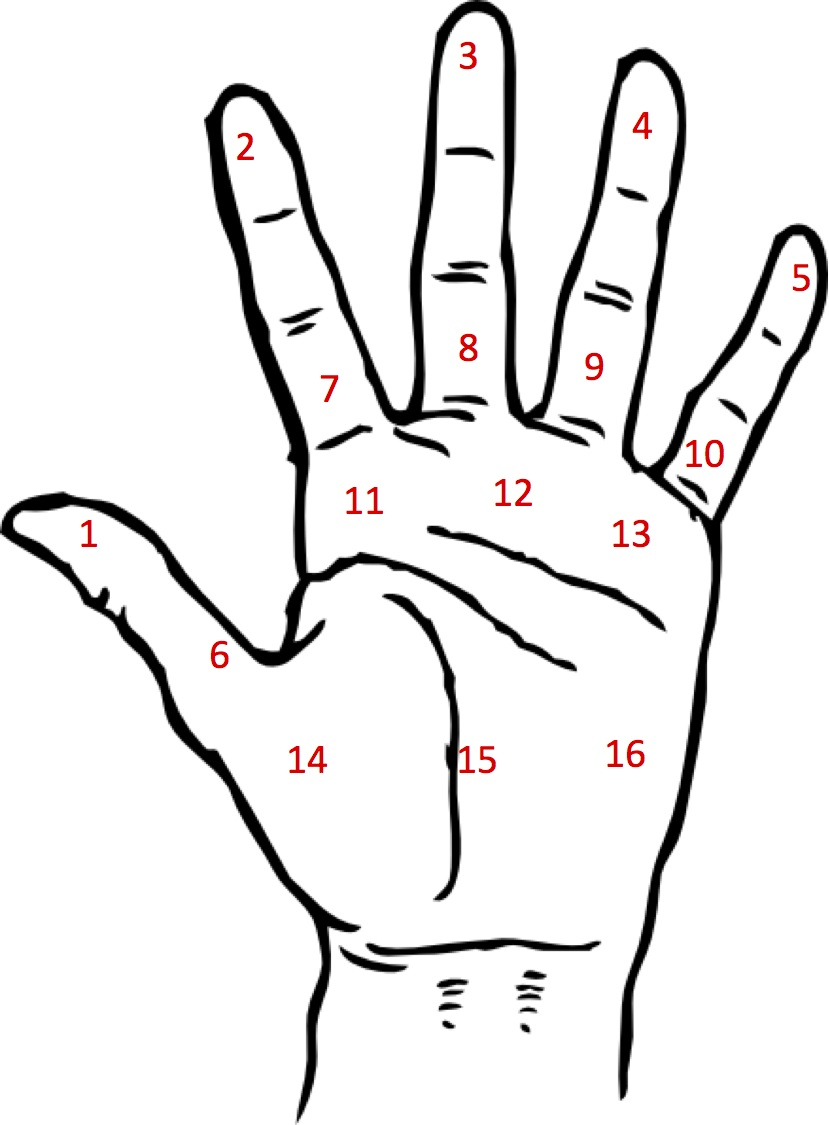
\includegraphics[width= 3.cm]{HandLocs_Left.jpg}}
\end{figure}
\end{column}
\end{columns}
\end{frame}

  \end{document}